\section{Results and Discussion}
\label{sec:results}
%
%Provide a summary of the performance on the previous year dataset.
%
%Discuss the results and any relevant issues.
%Qui sezione in cui esporre il lavoro vero e proprio: scenario di base ed evoluzione in base ai tentativi.
%Elenco puntato per punti di lavoro osservati: query expansion/lavoro sui sinonimi, presenza di spam e tentativi di eliminarlo, implementazione di re-ranking e tecniche NLP/NER.
%Ogni punto: come lo si è rilevato/concepito, approccio teorico ed implementazione, risultati ottenuti e brevi considerazioni (brevi perché c'è sez 5 apposita).
As aforementioned, it can be noted how work on the French corpus has been largely favoured.
Due to the fact that the English document and query set were obtained by translation of the French ones, the former batch contains a lot of translation-induced noise which strongly interferes with the goal of setting up an effective IR system. This was already seen from table \ref{tab:qtransl}.

\par Another related issue is document and queries not being translated homogeneously. As an example, in Table \ref{tab:nonuntransl} we report a couple consisting of a query and a highly relevant document and their translations.
\begin{table}[h!]
  \caption{Non-uniform translation example}
  \label{tab:nonuntransl}
  \centering
  \begin{tabular}{|l|l|l|}
    \toprule
    Item ID&French&English\\
    \midrule
    q0622311 & bourse de l emploi public & Public Employment Exchange\\
doc062200210641 & "Sélectionnée par Emploi Public" & "Selected by Public servant"\\
  \bottomrule
\end{tabular}
\end{table}
Such a translation, while semantically correct, makes it harder for the IR system to correctly match the document to the query.
\par Moreover, by comparing our base French and base English systems we observed consistently worse performance on the latter (see Table \ref{tab:sysperf}), while employing for the two systems essentially the same techniques (adapted to the respective languages).
\par

\begin{table}[h!]
  \caption{Systems performance overview}
  \label{tab:sysperf}
  \centering
  \begin{tabular}{|l|l|l|l|l|l|}
    \toprule
    System name & Language & NDCG & MAP & Recall@1000 & CLEF?\\
    \midrule
    BM25FRENCHNOENG & French & 0.3799 & 0.2139 & 0.8397 & No\\
    BM25FRENCHSPAM & French & 0.3623 & 0.2067 & 0.7648  & Yes\\
    BM25FRENCHBASE & French & 0.3812 & 0.2146 & 0.8451 & Yes\\
    BM25FRENCHBOOSTURL & French & 0.3815 & 0.2152 & 0.8421 & Yes\\
    BM25FRENCHRERANK100 & French & 0.3657 & 0.1960 & 0.8437 & Yes\\
    BM25TRANSLATEDQUERIES & Both & 0.3037 & 0.1523 & 0.7437 & Yes\\
    BaseSystem (base English system) & English & 0.2944 & 0.1505 & 0.7022 & No\\
  \bottomrule
\end{tabular}
\end{table}

\par Overall, the best system for all metrics is the \textit{BM25FRENCHBOOSTURL}. This particularly good performance can be due to the URL tokenizing system helping with queries  expressing \textit{ad hoc search} and \textit{known item search}. In this scope, keywords contained inside the URL are good indicators of page content: most of the time, while looking for a particular service or a website, the best match contains its name in the page URL, since those are more likely to be official websites and sources. Furthermore, considering the fact that some documents were rich of repetitions and useless symbols, considering the URLs in the search phase allowed us to distinguish more between real relevant documents and outliers.

\par Another thing to observe is the \textit{BM25TRANSLATEDQUERIES} performance in comparison to \textit{BaseSystem}. When compared to base French systems, the results highlight how difficult query translation is, and the different results between the two denote how using a different translator may substantially influence output.
This variance in results confirms how translation adds significant noise that interferes with the system IR-wise improvement process.

\par The \textit{BM25FRENCHRERANK100} system instead doesn't work as expected. In particular we were expecting to increase the nDCG by reranking the first 100 documents but this metric actually decreases. This can be due to the fact that by recreating the index based only on the top-100 documents the terms statistic changes and the new statistics favors the documents that are not considered relevant in the ground-truth.
\par To implement the reranking we thought about using some machine learning and/or deep learning techniques (Learn To Rank, LTR) but we were worried about the fact that since we had only a small number of relevance feedback for the training topics, then the resulting system would overfit on the training data.
\par
Figure \ref{fig:prcurve} shows the interpolated precision-recall curve for the two best performing systems.
\begin{figure}[h]
    \centering
    \includegraphics[scale=0.8]{figure/curve.eps}
    \caption{Interpolated precision-recall curve}
    \label{fig:prcurve}
\end{figure}
